% 流形
% 拓扑|流形|欧几里得

\pentry{拓扑空间\upref{Topol}}

\textbf{实流形(real manifold)} 是一种拓扑空间, 其每个点都有一邻域与与欧几里得空间中的开集同胚 (homomorphic).如果这些欧几里得空间是$n$维的, 那么就叫做$n$维流形. 因此,一个实流形可以看成是我们熟知的欧几里得空间 “拼接” 而成的.

\subsection{拓扑流形}

\begin{definition}{图和图册}\label{Manif_def1}
设$N$是一个拓扑空间,满足Hausdorff分离性以及第二可数性\footnote{拓扑空间如果有一个可数拓扑基(即一个拓扑基,包含最多$\aleph_0$个基本开集),则称之为第二可数的.}.如果存在开集$U\in\mathcal{T}_N$和一个正整数$n$,使得$U$同胚于$\mathbb{R}^n$,同胚映射为$\varphi:U\rightarrow\mathbb{R}^n$,那么称$(U,\varphi)$是$N$上的一张\textbf{图(chart)}.如果图的一个集合$\mathcal{A}=\{(U_\alpha, \varphi_\alpha)\}$覆盖了$N$,即$\bigcup\{U_\alpha\}=N$,那么称这个集合$\mathcal{A}$是一个\textbf{图册(atlas)}.
\end{definition}

图$(U, \varphi)$可以看成是给$U$中各点$x$赋予了一个坐标值$\varphi(x)$.

\begin{definition}{实拓扑流形}\label{Manif_def2}

设$N$是一个\textbf{道路连通的}拓扑空间,满足Hausdorff分离性以及第二可数性,且有一个图册$\mathcal{A}$,则称$(N, \mathcal{A})$是一个\textbf{实拓扑流形(real topological manifold)}.

\end{definition}

从这些定义可看到,流形是“局部地”和欧几里得空间同胚的数学对象.低维欧几里得空间可以很方便地用我们的几何直觉来理解,大大方便了建立对于流形的直觉.

要注意的是,以上定义只要求了流形的每个点附近都有领域,使之局部地同胚于欧几里得空间,这样的流形被称为拓扑流形,但并不是我们将在微分几何中讨论的重点;我们将来讨论的重点概念是“光滑流形”.

\begin{example}{$S^n$流形}

$n$维球面$S^n$都是实流形.
\begin{itemize}
\item 记$S^1=\{(\cos{2\pi t},\sin{2\pi t})\in\mathbb{R}^2|t\in[0, 1]\}$,那么我们可以通过挖去一个点后使用正切函数来构造图:$U=S^1-\{(1,0)\}=\{(\cos{2\pi t},\sin{2\pi t})\in\mathbb{R}^2|t\in(0, 1)\}$可以同胚于$\mathbb{R}$,同胚映射为$\varphi(\cos{2\pi t},\sin{2\pi t})=\tan{\pi t-\pi/2}$;类似地,$V=S^1-\{(-1, 0)\}=\{(\cos{2\pi t},\sin{2\pi t})\in\mathbb{R}^2|t\in(-1/2, 1/2)\}$也可以同胚于$\mathbb{R}$,同胚映射为$\phi(\cos{2\pi t},\sin{2\pi t})= \tan{\pi t}$.这样一来,$\{(U, \varphi), (V, \phi)\}$就是$S^1$的两个图的集合,并且覆盖$S^1$,因此这个集合是一个图册,从而得出$S^1$是一个实拓扑流形.
\item 类似地,从$S^n$中分别挖去两个不同的点所得到的$U$和$V$都可以同胚于$\mathbb{R}^n$,从而得到图册.


\end{itemize}

\end{example}

\begin{example}{莫比乌斯带}
将莫比乌斯带表示为矩形纸带两边扭转后粘合,我们可以将其用如图所示的$5$个开集$U_i$覆盖,每个开集都同胚于$\mathbb{R}^2$,因此我们可以利用它们来构建一个含有$5$个图的图册.
\begin{figure}[ht]
\centering
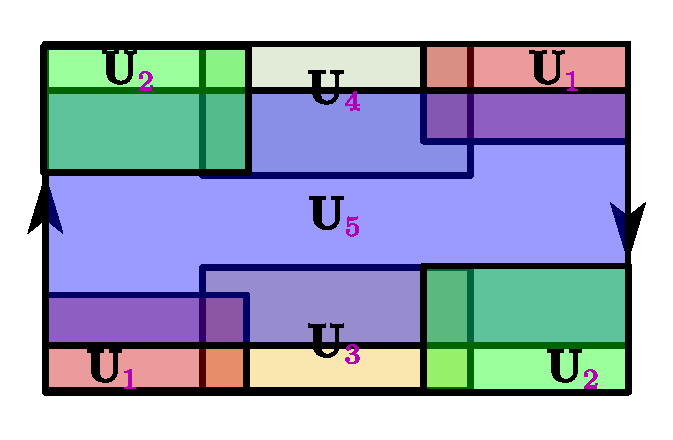
\includegraphics[width=5cm]{./figures/Manif_1.pdf}
\caption{莫比乌斯带和覆盖它的五个开集.注意$U1$(红色)和$U2$(绿色)在图示中有“两块”区域,当然它们实际上是相连的.} \label{Manif_fig1}
\end{figure}
\end{example}

\subsection{光滑流形}

考虑一个拓扑流形$N$的两个图$(U, \varphi)$和$(V, \phi)$.如果$U\cap V\not=\varnothing$,那么在$U\cap V$中的每个点就有两套坐标;当然,也可以把$\varphi\circ\phi^{-1}:\phi(V)\rightarrow\varphi(U)$和$\phi\circ\varphi^{-1}:\varphi(U)\rightarrow\phi(V)$看成$\mathbb{R}^n$的开子集上的多元向量值函数.只要这个函数是可以任意进行微分的,就能方便我们研究.

\begin{definition}{光滑函数}
设$f:\mathbb{R}^n\rightarrow\mathbb{R}$是一个$n$元函数,如果$\frac{\partial^{k_1+k_2+\cdots+k_n}}{\partial^{k_1}x^1\partial^{k_2}x^2\cdots\partial^{k_n}x^n} f$在一点$x\in\mathbb{R}^n$处对于任意非负整数$k_i$成立,即$f$的任意阶偏导数存在,那么称$f$在$x$处光滑;如果$f$处处光滑,也称它是一个\textbf{光滑函数(smooth function)},记为$C^\infty$的函数.如果向量值函数的各分量函数都是光滑函数,那么也称这个向量值函数是一个\textbf{光滑映射(smooth map)}.
\end{definition}

当一个函数的$m$阶偏导数存在并且连续时,我们说它是$C^m$的,因此任意阶偏导数存在时自然被记为$C^\infty$.今后我们将“光滑”和$C^\infty$视为同义词,不加区分.

需要注意的是,光滑和解析不是等价的概念.解析函数一定光滑,但光滑函数不一定解析,一个典型例子是\autoref{SmthM_ex1}~\upref{SmthM}.可参考幂级数\upref{anal}.

\begin{definition}{相容}
考虑一个拓扑流形$N$的两个图$(U, \varphi)$和$(V, \phi)$.如果$U\cap V\not=\varnothing$,且$\varphi\circ\phi^{-1}:\phi(V)\rightarrow\varphi(U)$和$\phi\circ\varphi^{-1}:\varphi(U)\rightarrow\phi(V)$都是光滑映射,那么我们称这两个图是\textbf{相容的(compatible)}.
\end{definition}

从拓扑流形例子可以看出,同一个拓扑空间$N$可以有不同的图册,对应的虽然是同一空间,但按照定义却是不同流形.这意味着流形不仅仅是指空间$N$本身,还指它的局部坐标系结构.这样把拓扑流形分类通常是无意义的,实际上我们需要一个更为统一的研究对象,那就是光滑流形.我们接连使用以下两个定义来定义光滑流形.

\begin{definition}{极大图册}
设$(N, \mathcal{A})$是一个拓扑流形.如果$N$的任何一个图,满足“只要它和$\mathcal{A}$中\textbf{所有图}都相容,它就一定在$\mathcal{A}$中”,那么就称$\mathcal{A}$是一个极大图册.
\end{definition}

\begin{definition}{光滑流形}
拥有极大图册的拓扑流形,被称为一个\textbf{光滑流形(smooth manifold)}.光滑流形的图册,被称为该流形上的一个\textbf{微分结构(differential structure)}.
\end{definition}

将以上定义中的$\mathbb{R}^n$替换为$\mathbb{C}^n$,图册中的"光滑映射"替换为"复解析映射", 我们就得到复流形的定义:

\begin{definition}{复流形}

将\autoref{Manif_def1} 中图的定义限定为到$\mathbb{C}^n$中开集的同胚, 图册的定义限定为$\mathbb{C}^n$开集之间的复解析映射,那么\autoref{Manif_def2} 中所定义的实光滑流形就变成了\textbf{复流形(complex manifold)}.

\end{definition}


这就是我们将来讨论的主要对象了.今后如无特别说明,本书中“流形”一词都特指“光滑流形”.

通常,为了方便,我们也会将流形$(N, \mathcal{A})$简单记为$N$.





